\documentclass{article}
\usepackage[utf8]{inputenc}
\usepackage[spanish]{babel}
\usepackage{graphicx}
\usepackage{float}
\usepackage{hyperref}

\title{Práctica 4 - Segunda Parte\\Servidor IoT}
\author{Noelia Escalera Mejías}

\begin{document}
	\maketitle
	\section{Explicación del método de comunicación}
	Para comunicar el servidor con 'vista\_usuario.html' y con 'sensores.html' lo hemos hecho a través de socket.io. En el servidor tenemos:
	\begin{figure}[H]
		\centering
		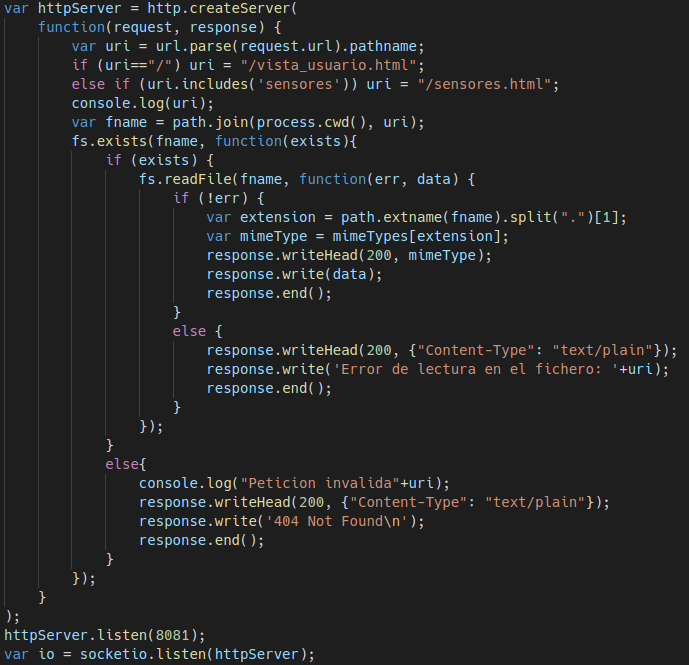
\includegraphics[totalheight=11.7cm]{img/39.png}
	\end{figure}
	Creamos un servidor http y redireccionamos a la página que nos convenga. Luego en los clientes ya nos conectamos de la siguiente manera:
	 \begin{figure}[H]
	 	\centering
	 	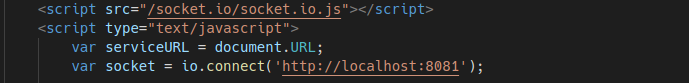
\includegraphics[totalheight=1.5cm]{img/40.png}
	 \end{figure}
 	Nos conectamos al puerto 8081, ya que el 8080 dio problemas. Básicamente para cooperar entre nodos, se ha hecho uso de los emit y de los on. Cuando es necesario que emitan todos los sockets, ser hace un io.sockets en vez de que lo emita solo el cliente. Esto se va a ver más claramente a continuación en la explicación de los métodos.
	\section{Explicación del funcionamiento de la aplicación y de sus métodos}
	Al entrar a la aplicación, nos encontramos esto:
	\begin{figure}[H]
		\centering
		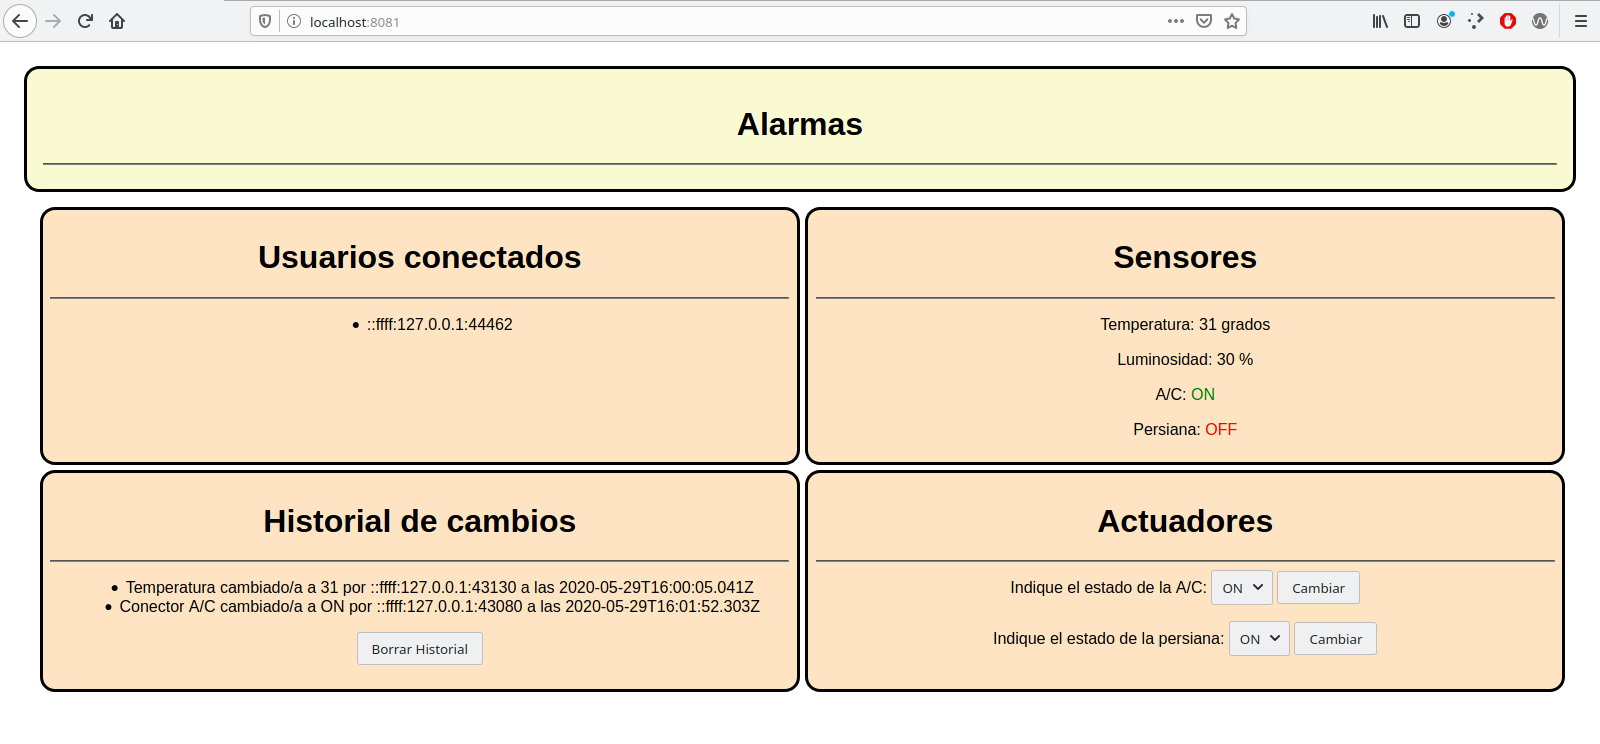
\includegraphics[totalheight=6cm]{img/1.png}
	\end{figure}
	Y si nos conectamos al formulario:
	\begin{figure}[H]
		\centering
		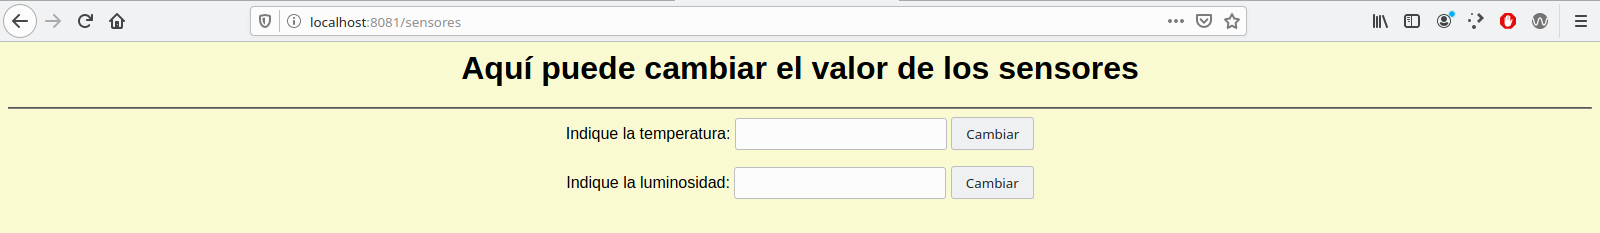
\includegraphics[totalheight=1.9cm]{img/2.png}
	\end{figure}
	Vamos a ir explicando los módulos uno por uno:
	\subsection{Usuarios conectados}
	Muestra los usuarios conectados al sistema en tiempo real, también cuentan los que estén conectados al formulario:
	\begin{figure}[H]
		\centering
		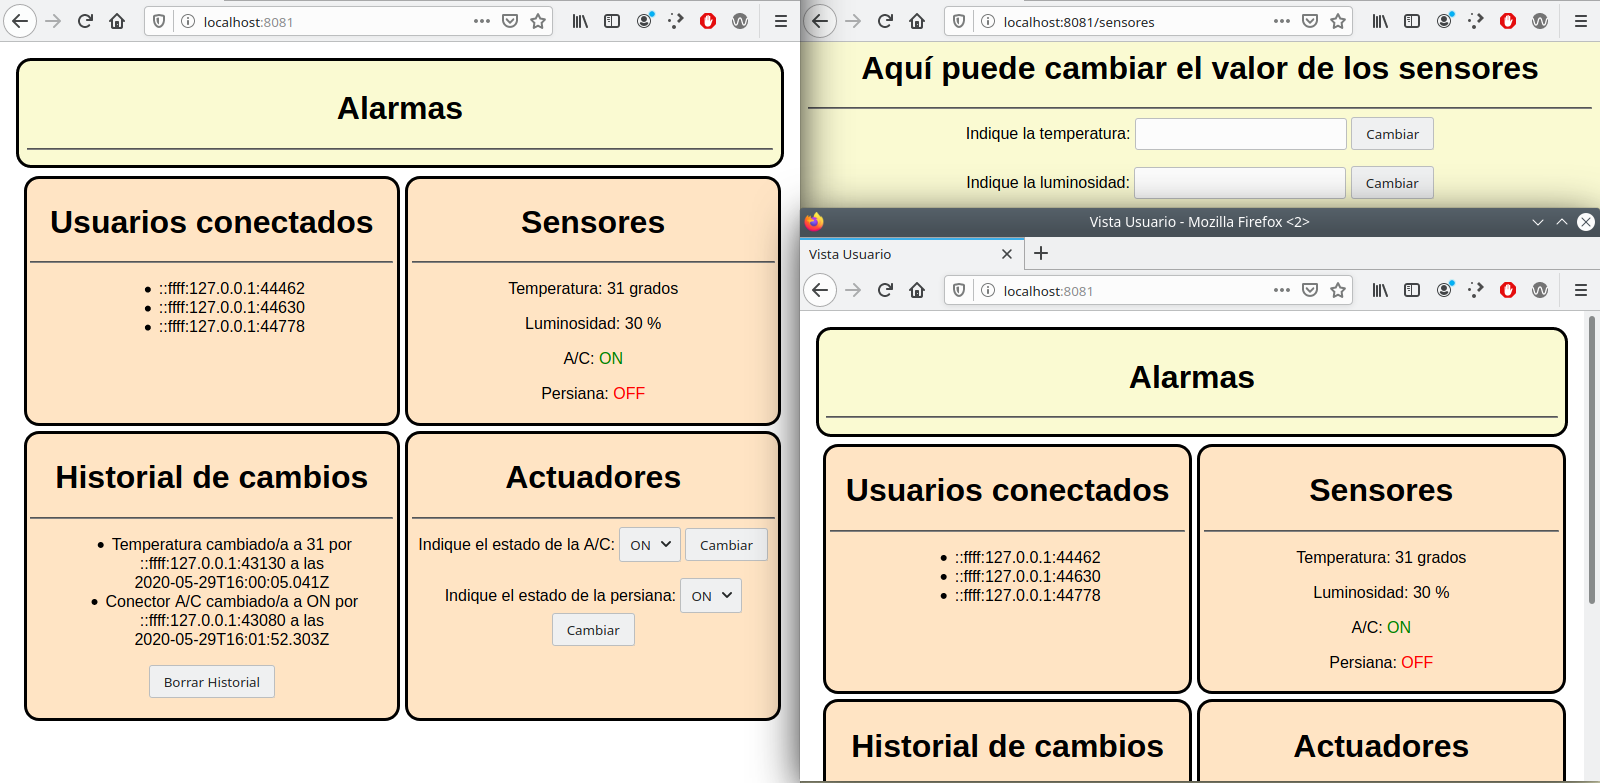
\includegraphics[totalheight=6cm]{img/3.png}
	\end{figure}
	Esto está directamente basado en el Ejemplo 4 del guión. Aquí tenemos el método del servidor, cada vez que un usuario se conecta, lo comunica por consola al igual que cuando se desconecta:
	\begin{figure}[H]
		\centering
		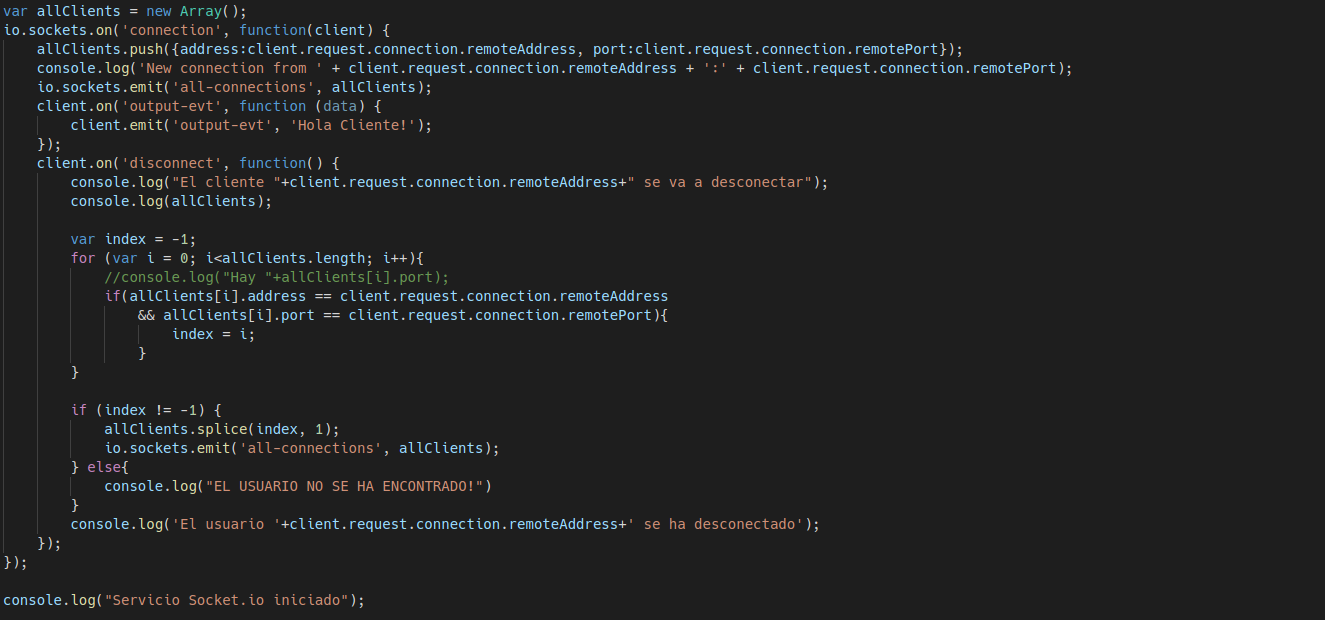
\includegraphics[totalheight=6cm]{img/4.png}
	\end{figure}
	Este método emite además una llamada a 'all-connections', que se recoge en el cliente:
	\begin{figure}[H]
		\centering
		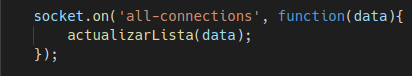
\includegraphics[totalheight=2.5cm]{img/5.png}
	\end{figure}
	Como vemos, se llama a la función actualizarLista, veamos su código:
	\begin{figure}[H]
		\centering
		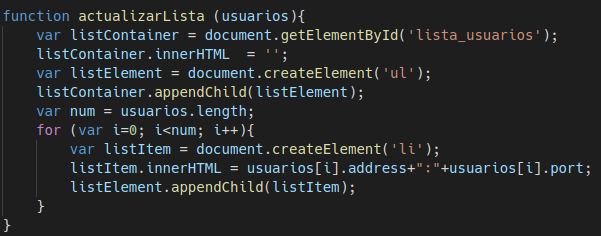
\includegraphics[totalheight=5.3cm]{img/6.png}
	\end{figure}
	Esta función recorre el array de usuarios y va imprimiendo su dirección y su puerto en el sitio correspondiente.
	\subsection{Sensores y actuadores}
	El campo sensores muestra el estado actual de todas las variables del sistema en tiempo real. El campo actuadores permite accionar el A/C y la persiana. Podemos modificar el valor de la luminosidad y la temperatura mediante el formulario. He aquí un ejemplo:
	\begin{figure}[H]
		\centering
		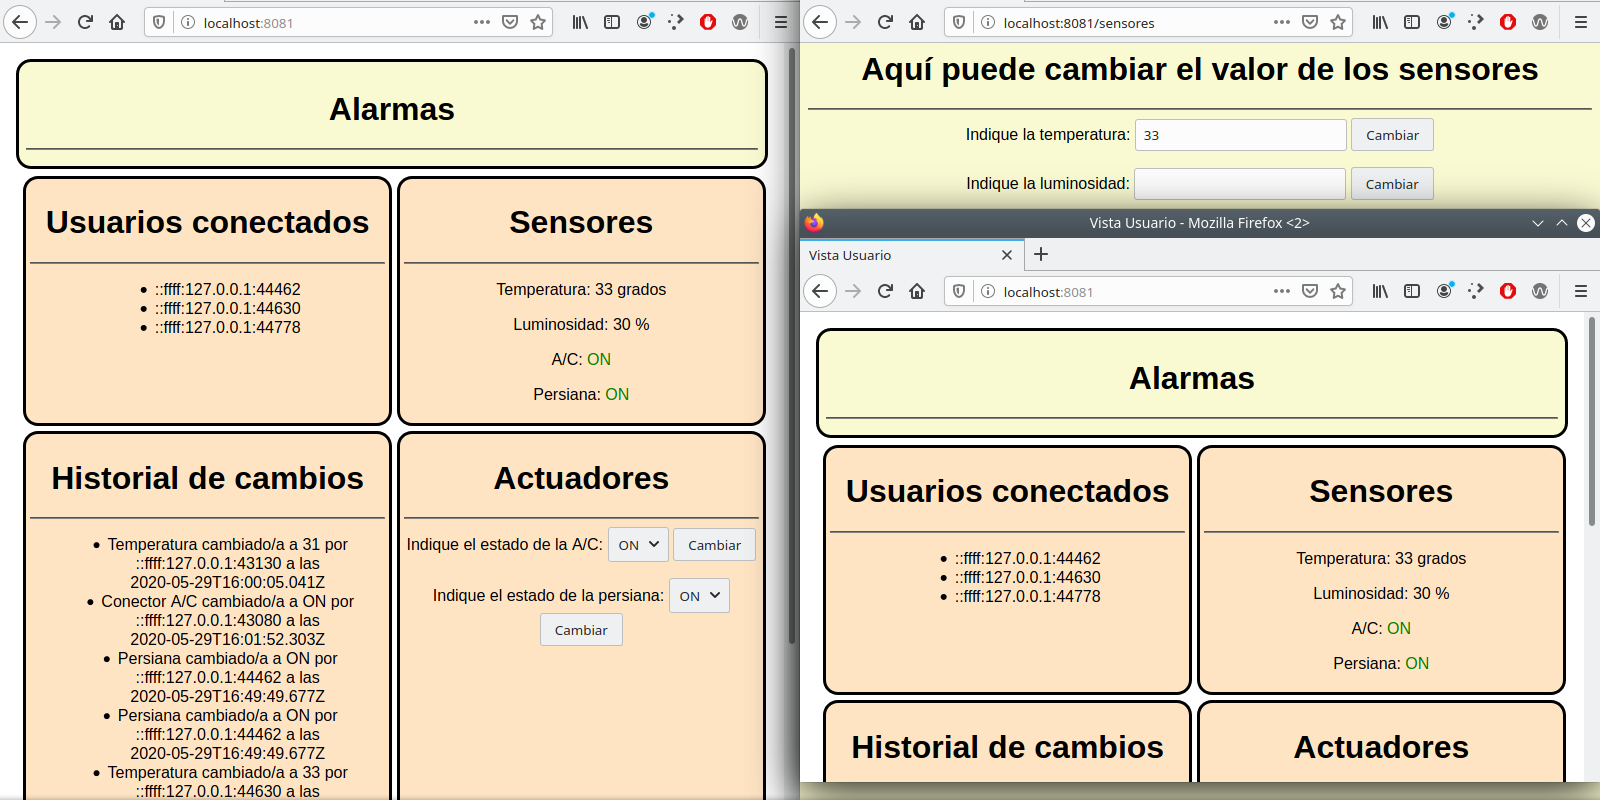
\includegraphics[totalheight=6cm]{img/7.png}
	\end{figure}
	Veamos como se consigue esto. Básicamente tenemos una colección de MongoDB para cada variable. Cada vez que modifiquemos el valor de uno de los sensores, se insertará una nueva fila en la colección del sensor. Como los métodos son prácticamente iguales en las cuatro variables vamos a ver los del A/C como ejemplo de actuador y los de Temperatura como ejemplo de sensor. Empecemos con los de A/C:
	\begin{figure}[H]
		\centering
		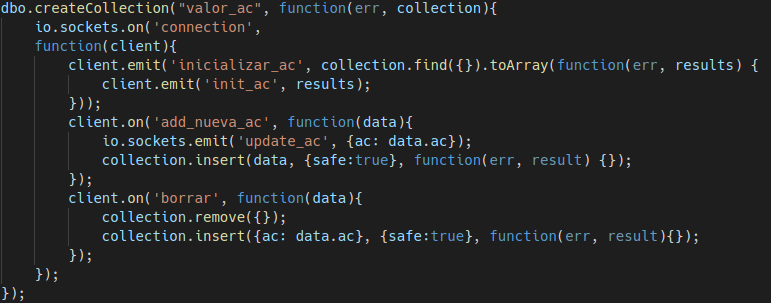
\includegraphics[totalheight=4.7cm]{img/8.png}
	\end{figure}
	Vamos a obviar por ahora 'borrar', que lo explicaremos con el historial de cambios. Nada más conectarse un cliente, se hará un emit de 'inicializar\_ac', que recogerá todas los datos de la colección y a continuación hará un emit de 'init\_ac'. Este emit será recogido en el cliente:
	\begin{figure}[H]
		\centering
		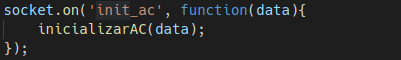
\includegraphics[totalheight=1.8cm]{img/9.png}
	\end{figure}
	Como vemos, simplemente llama a la funcion 'inicializarAC', a la que le pasa los datos recogidos de la consulta, veamos qué hace esta función:
	\begin{figure}[H]
		\centering
		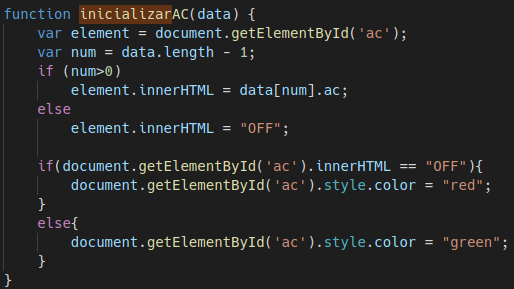
\includegraphics[totalheight=6.7cm]{img/10.png}
	\end{figure}
	Primero va a comprobar que haya algún valor anteriormente, si no pondrá por defecto a 'OFF', sino, pues pondrá el valor de la última fila insertada, ya que será el valor más reciente que tuvo la variable antes de apagarse el sistema. También pondrá el texto en rojo o verde, dependiendo de si está encendido o apagado.
	
	En los métodos del servidor veíamos un client.on('add\_nueva\_ac'):
	\begin{figure}[H]
		\centering
		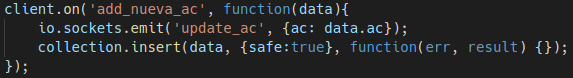
\includegraphics[totalheight=1.65cm]{img/11.png}
	\end{figure}
	Podemos ver que hace un emit a todos los sockets de 'update\_ac' y luego inserta los datos que le pasamos a la colección. ¿Pero desde dónde se llama a esta función? Pues se llama cuando pulsamos cambiar en el formulario del A/C:
	\begin{figure}[H]
		\centering
		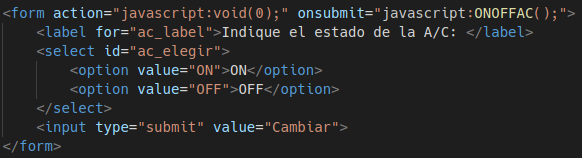
\includegraphics[totalheight=3.3cm]{img/12.png}
	\end{figure}
	\begin{figure}[H]
		\centering
		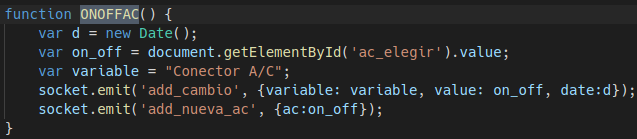
\includegraphics[totalheight=2.7cm]{img/13.png}
	\end{figure}
	Al enviar el formulario, llamamos a la función 'ONOFFAC()'. Esta función es la que hace el emit de 'add\_nueva\_ac' y le manda el nuevo valor del A/C, metiéndolo en la colección desde el servidor, además hace un emit de 'add\_cambio', que luego explicaremos en detalle, pero adelantamos que tiene que ver con el historial.
	
	Vamos a ver ahora los métodos de Temperatura:
	\begin{figure}[H]
		\centering
		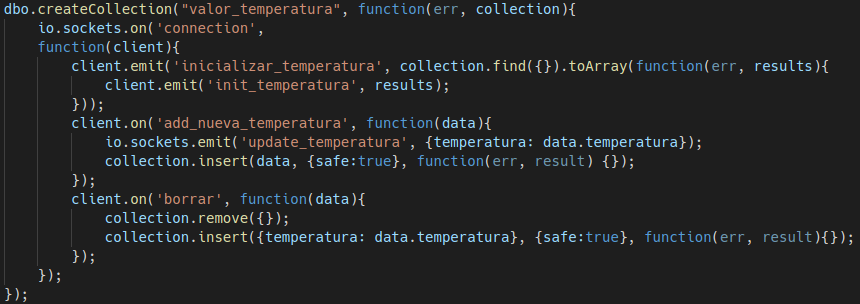
\includegraphics[totalheight=4.4cm]{img/14.png}
	\end{figure}
	Podemos observar que son los mismos que los de A/C, la diferencia es que la función que llama en este caso a 'add\_nueva\_temperatura' está en el archivo de 'sensores.html', ya que se llama desde el formulario que hay ahí:
	\begin{figure}[H]
		\centering
		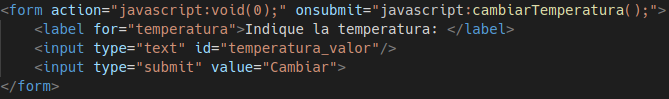
\includegraphics[totalheight=1.85cm]{img/15.png}
	\end{figure}
	\begin{figure}[H]
		\centering
		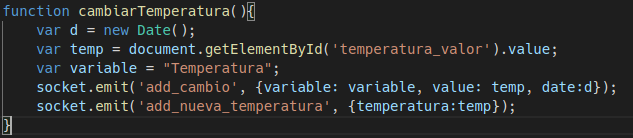
\includegraphics[totalheight=2.75cm]{img/16.png}
	\end{figure}
	\subsection{Historial de cambios}
	El historial de cambios recoge todos los cambios que se han hecho en las medidas, el usuario que las realizó y la fecha:
	\begin{figure}[H]
		\centering
		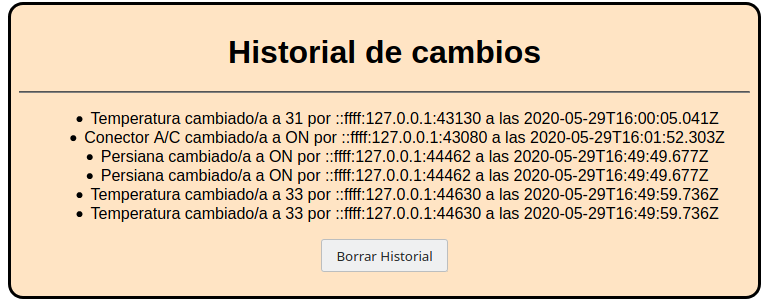
\includegraphics[totalheight=5cm]{img/17.png}
	\end{figure}
	Tenemos una colección que almacena todos estos datos (variable cambiada, nuevo valor, usuario y fecha). Esto es lo que tenemos en el servidor:
	\begin{figure}[H]
		\centering
		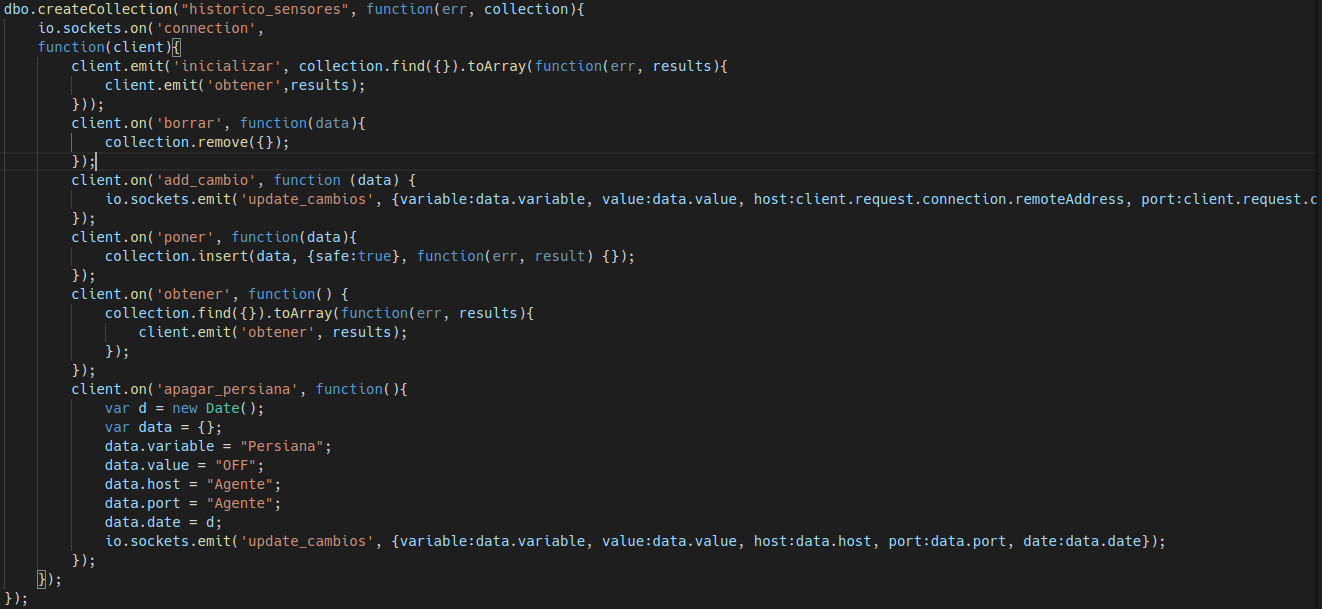
\includegraphics[totalheight=6cm]{img/18.png}
	\end{figure}
	Nada más conectarse un cliente se hace un emit de 'inicializar', que carga todo el historial, y se hace un emit de 'obtener', al que se le pasan estos datos (como vemos es muy similar a lo de los sensores). El emit de 'obtener' se captura en el cliente:
	\begin{figure}[H]
		\centering
		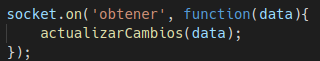
\includegraphics[totalheight=1.6cm]{img/19.png}
	\end{figure}
	Esto llama a la función actualizarCambios:
	\begin{figure}[H]
		\centering
		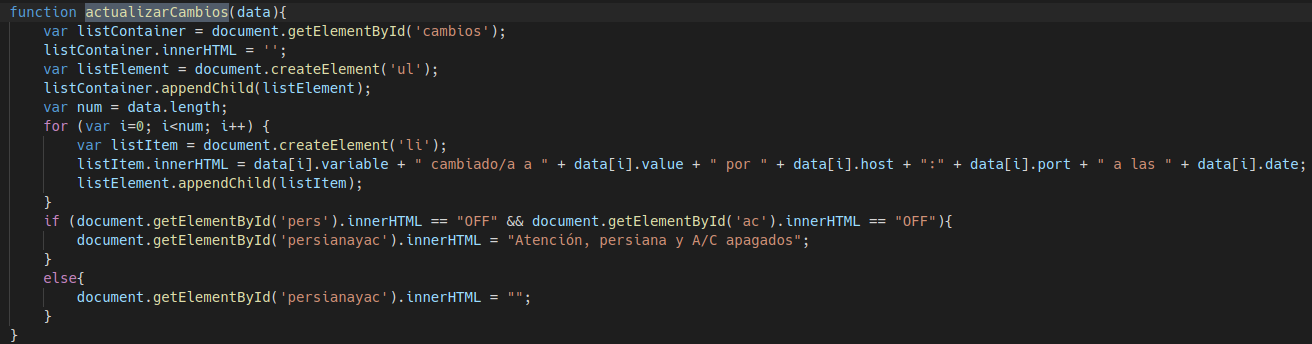
\includegraphics[totalheight=3.2cm]{img/20.png}
	\end{figure}
	Básicamente recorre todos los cambios y los pone en el sitio indicado. También lanza una alarma si la persiana y el aire acondicionado están apagados. Veamos ahora qué es lo que hace el método 'borrar', que lo tenemos tanto aquí como en los sensores. Este método se llama cuando pulsamos el botón 'Borrar Historial':
	\begin{figure}[H]
		\centering
		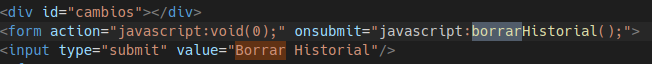
\includegraphics[totalheight=1.2cm]{img/21.png}
	\end{figure}
	\begin{figure}[H]
		\centering
		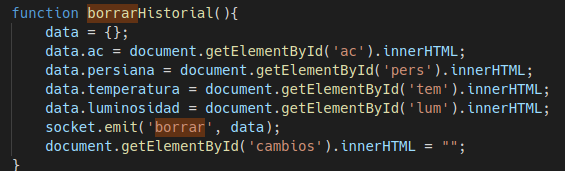
\includegraphics[totalheight=3.7cm]{img/22.png}
	\end{figure}
	Como vemos, guarda los valores actuales de las variables, hace un emit de borrar y deja el espacio del historial en blanco. Veamos lo que hacen los distintos borrar del servidor:
	\begin{figure}[H]
		\centering
		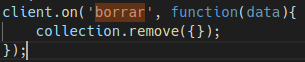
\includegraphics[totalheight=2.5cm]{img/23.png}
	\end{figure}
	En la colección de historial, simplemente borra todos los datos.
	\begin{figure}[H]
		\centering
		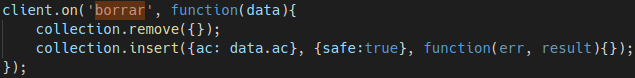
\includegraphics[totalheight=1.5cm]{img/24.png}
	\end{figure}
	En las colecciones de las variables, borra también los datos, pero vuelve a meter el último valor almacenado, que lo hemos pasado desde el cliente, esto nos sirve para que siempre quede un valor recordado.
	
	Vamos a ver ahora el método 'add\_cambio':
	\begin{figure}[H]
		\centering
		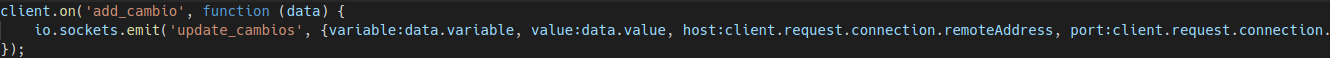
\includegraphics[totalheight=0.55cm]{img/25.png}
	\end{figure}
	'add\_cambio' ya vimos que se emitía cuando se cambiaba una variable, y le pasábamos la variable cambiada, su nuevo valor y la fecha. Al recibir este mensaje, todos los sockets emiten 'update\_cambios', al cual se le pasan todos estos datos, además de la ip y del puerto. Este método se escucha en el cliente:
	\begin{figure}[H]
		\centering
		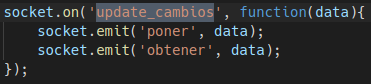
\includegraphics[totalheight=2.9cm]{img/26.png}
	\end{figure}
	Esta función hace emit de 'poner' y de 'obtener'. Ambos métodos se encuentran en el servidor:
	\begin{figure}[H]
		\centering
		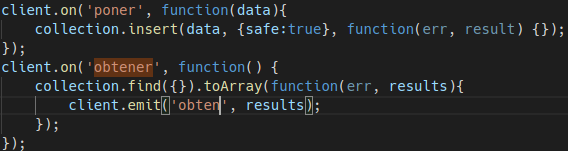
\includegraphics[totalheight=3.3cm]{img/27.png}
	\end{figure}
	'poner', inserta en la colección del historial el nuevo cambio. 'obtener' obtiene todos los cambios hasta ahora y emite 'obten', en este caso para el cliente:
	\begin{figure}[H]
		\centering
		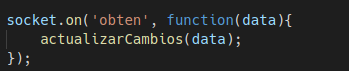
\includegraphics[totalheight=2.5cm]{img/28.png}
	\end{figure}
	Como vemos, este método simplemente llama a 'actualizarCambios' (función que ya hemos visto) para actualizar el historial.
	\subsection{Alertas}
	En esta sección se nos muestran las alertas del sistema, ya hemos visto una, que se activa cuando están apagadas tanto la persiana como el A/C y que se comprueba cuando se actualizan los cambios:
	\begin{figure}[H]
		\centering
		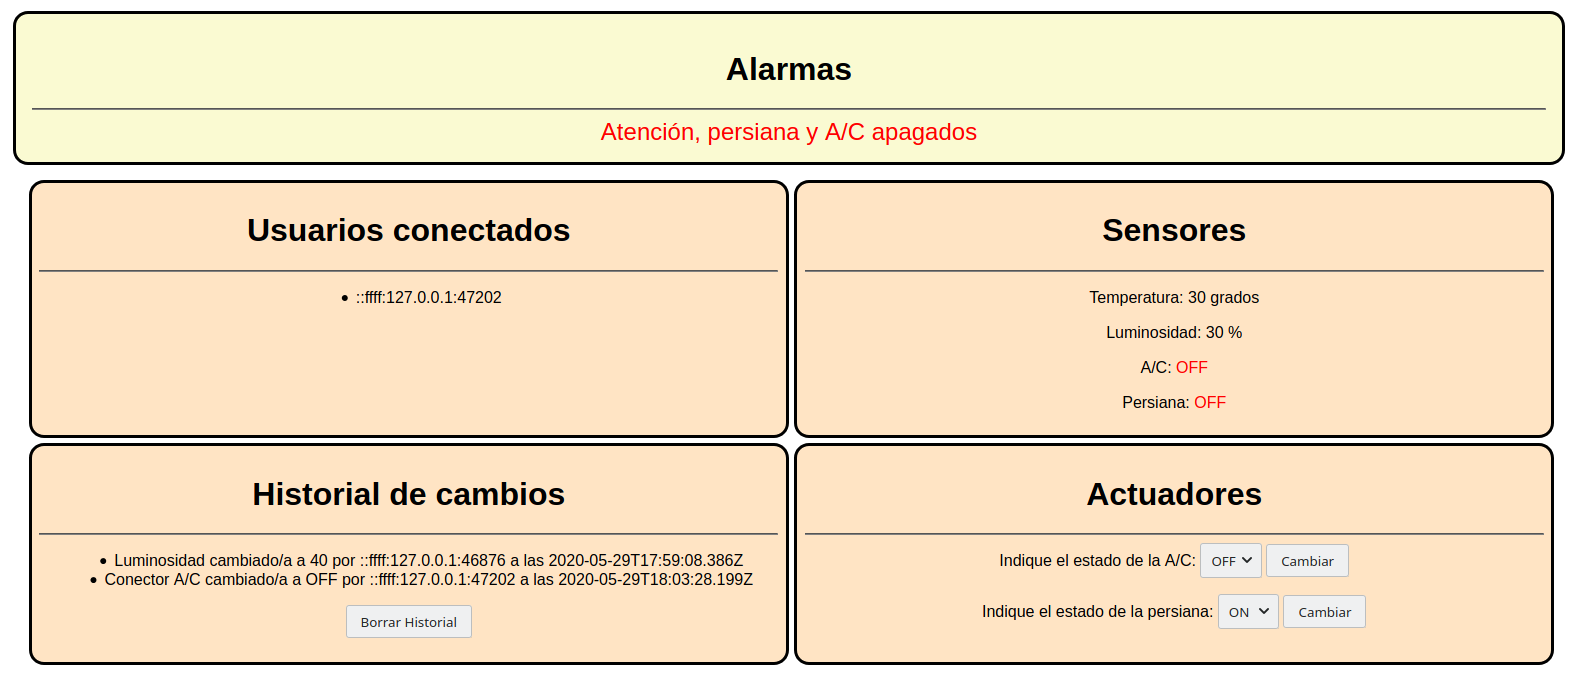
\includegraphics[totalheight=5cm]{img/29.png}
	\end{figure}
	Cuando una de las dos se enciende, la alarma cesa:
	\begin{figure}[H]
		\centering
		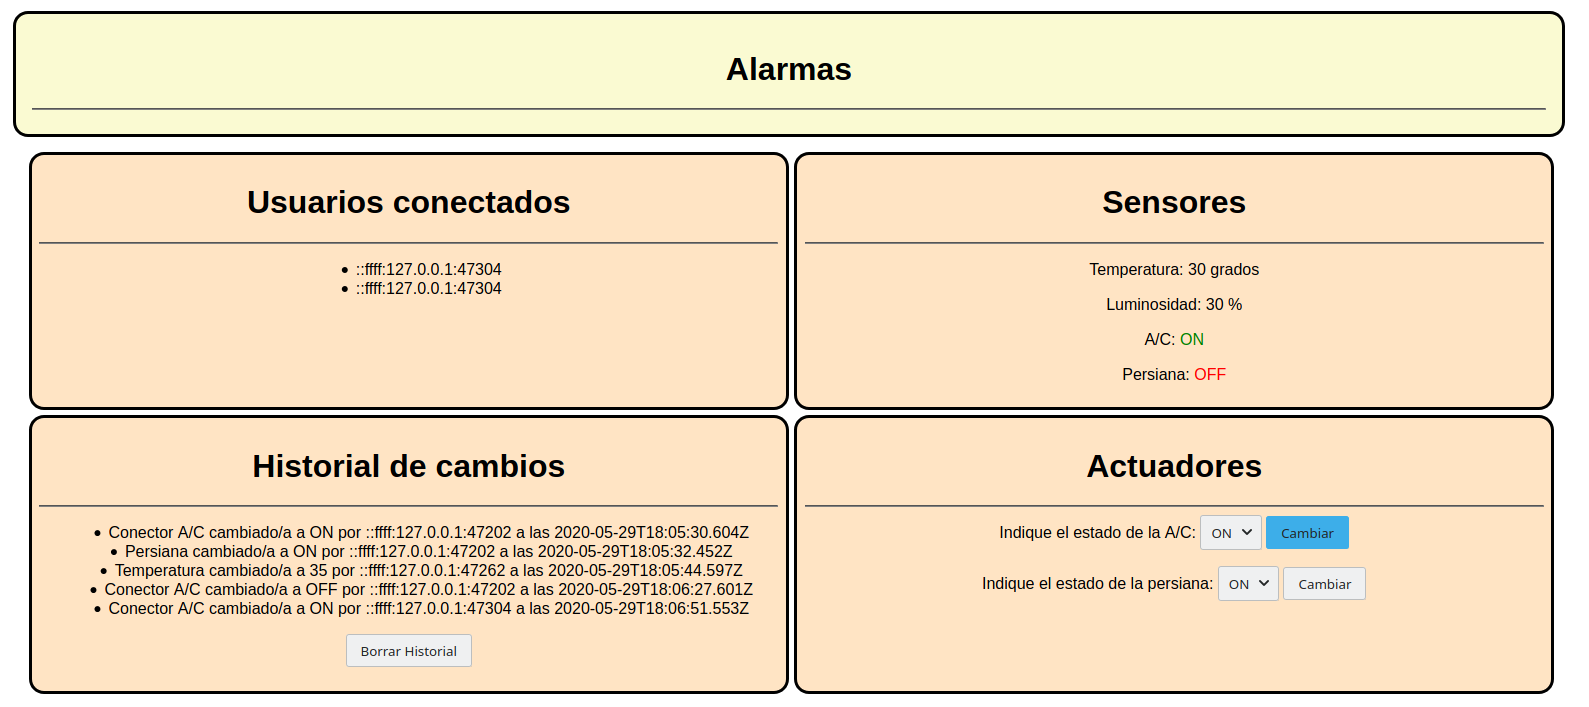
\includegraphics[totalheight=5cm]{img/30.png}
	\end{figure}
	Las otras alarmas que hay son cuando bien la temperatura, bien la luminosidad sobrepasan el límite (además la persiana se apaga automáticamente, y en el historial se recoge que lo ha hecho el agente):
	\begin{figure}[H]
		\centering
		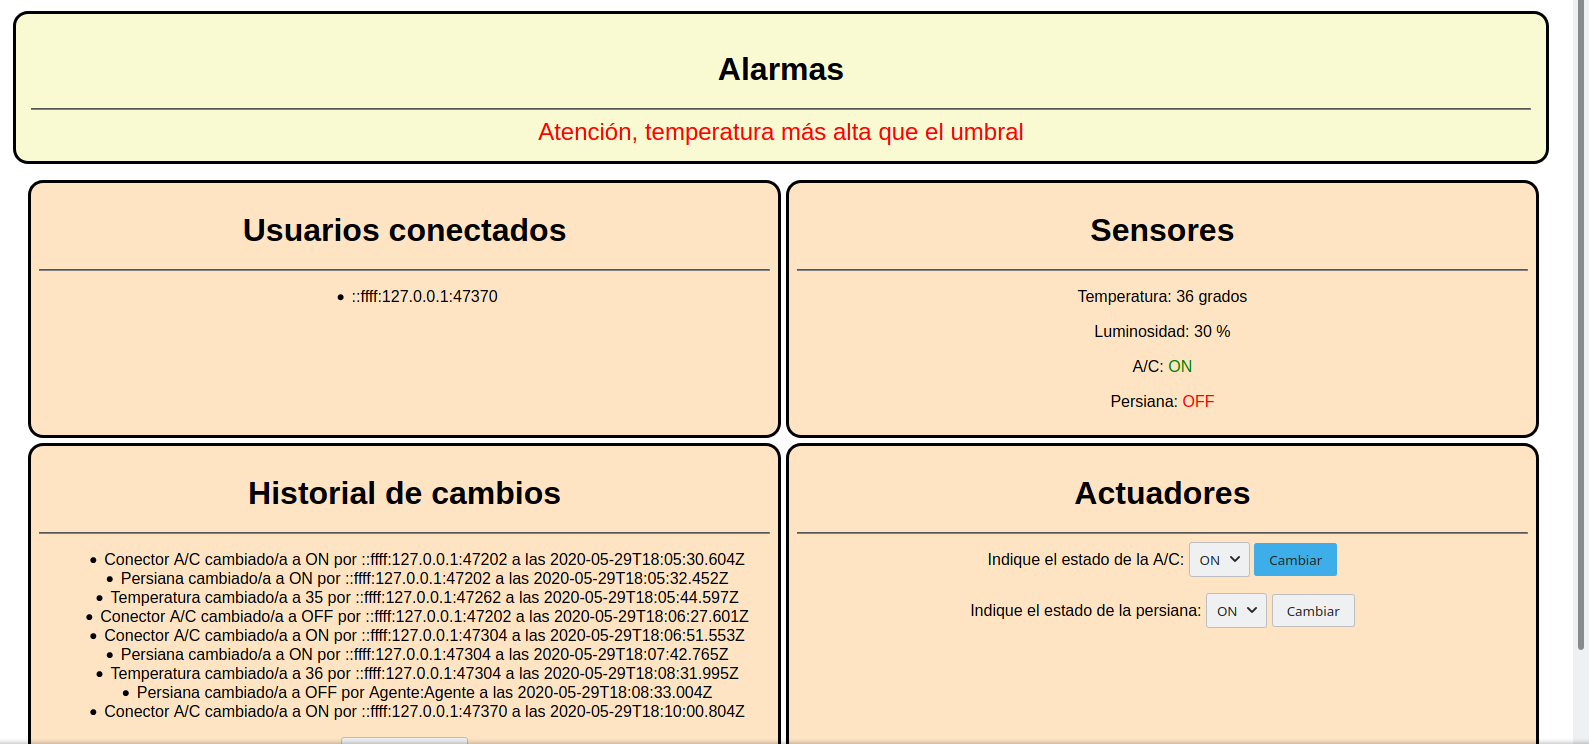
\includegraphics[totalheight=5cm]{img/31.png}
	\end{figure}
	Vamos a explicar esta alarma con la temperatura, con la luminosidad es igual.
	\begin{figure}[H]
		\centering
		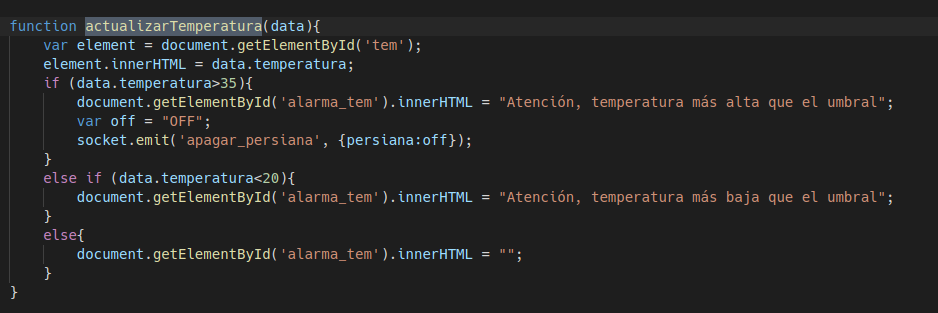
\includegraphics[totalheight=4.5cm]{img/33.png}
	\end{figure}
	\begin{figure}[H]
		\centering
		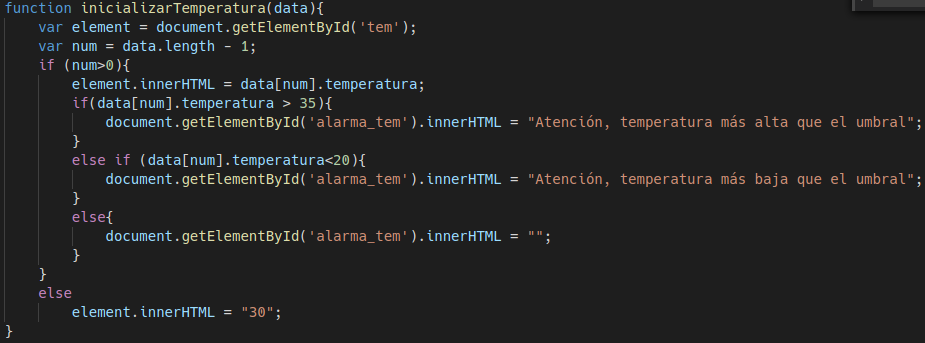
\includegraphics[totalheight=5cm]{img/34.png}
	\end{figure}
	Cuando bien inicializamos el sistema, o bien cuando actualizamos la temperatura/luminosidad, hay que comprobar si alguno de estos valores está por debajo o por encima del umbral. Si es el caso, se lanzará una alarma. Si se ha superado el umbral alto, además se hará un emit de 'apagar\_persiana'. Esto solo se hace en actualizar, ya que al inicializar se supone que ya ha habido un cambio anterior y por tanto ya se ha bajado la persiana. 'apagar\_persiana' lo tenemos en el servidor, en la parte del historial:
	\begin{figure}[H]
		\centering
		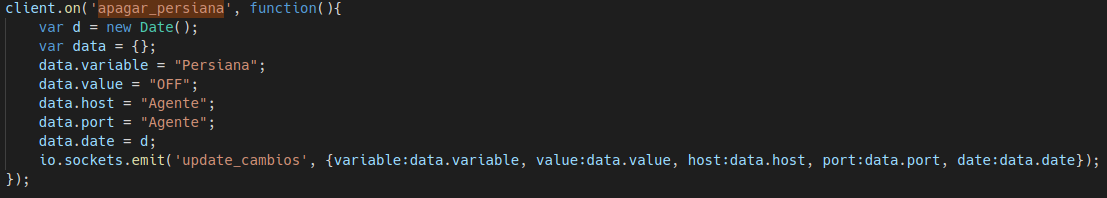
\includegraphics[totalheight=2.25cm]{img/35.png}
	\end{figure}
	Básicamente mandamos un cambio al historial, esta vez hecho por el agente. En los métodos de la colección de Persiana, también escuchamos 'apagar\_persiana':
	\begin{figure}[H]
		\centering
		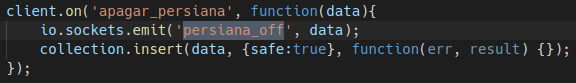
\includegraphics[totalheight=1.85cm]{img/36.png}
	\end{figure}
	Aquí hacemos que todos los sockets emitan 'persiana\_off' y se inserta en la colección de persiana el nuevo cambio. 'persiana\_off' tiene su socket.on en el cliente:
	\begin{figure}[H]
		\centering
		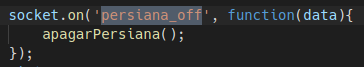
\includegraphics[totalheight=1.85cm]{img/37.png}
	\end{figure}
	\begin{figure}[H]
		\centering
		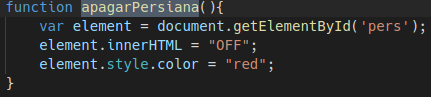
\includegraphics[totalheight=3cm]{img/38.png}
	\end{figure}
	Este método llama a 'apagarPersiana', que informa a los usuarios del cierre de la persiana.
\end{document}